\clearpage
\appendix

\section*{Appendix}
\addcontentsline{toc}{section}{Appendix}

\subsection*{A. Problem 1 Implementation}
\addcontentsline{toc}{subsection}{A. Problem 1 Implementation}

Implementation details for the Orthogonal Matching Pursuit algorithm.

\clearpage

This appendix contains implementation details for the three problems.

\subsection*{B. Problem 2 Implementation}
\addcontentsline{toc}{subsection}{B. Problem 2 Implementation}

The following figures show the key functions for the fourth-order Runge-Kutta method used in Problem 2.

\begin{figure}[H]
\centering
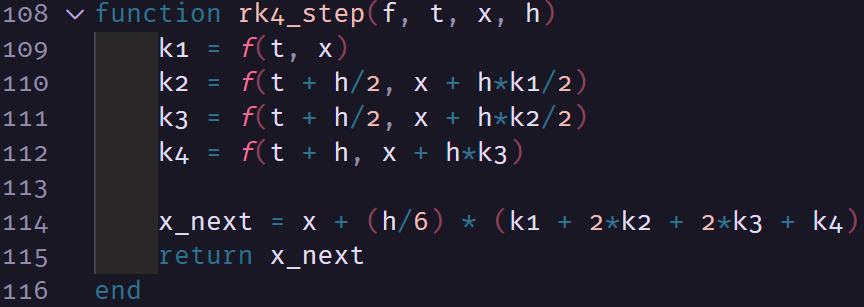
\includegraphics[width=0.9\textwidth]{figures/p02-code-rk4-step-function.png}
\caption{RK4 Step Function: Implements a single step of the fourth-order Runge-Kutta method with the four-stage computation ($k_1, k_2, k_3, k_4$).}
\label{fig:p02_rk4_step}
\end{figure}

\begin{figure}[H]
\centering
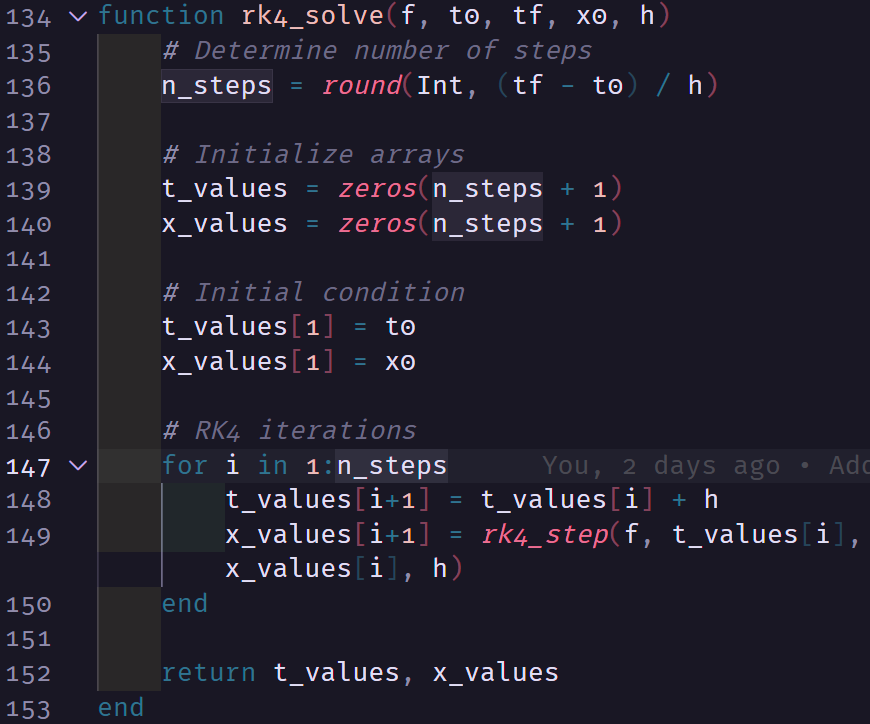
\includegraphics[width=0.9\textwidth]{figures/p02-code-rk4-solve-function.png}
\caption{RK4 Solve Function: Complete solver that iterates through all time steps, maintaining arrays of solution values.}
\label{fig:p02_rk4_solve}
\end{figure}

\begin{figure}[H]
\centering
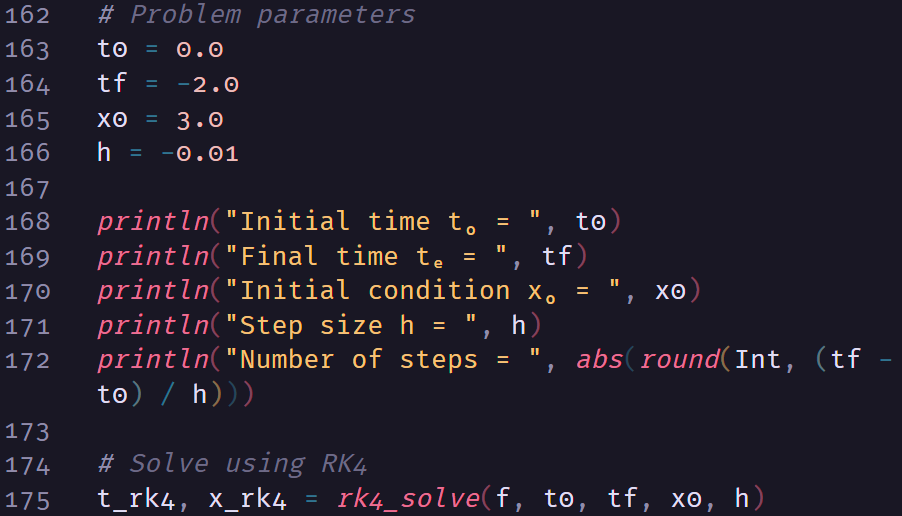
\includegraphics[width=0.9\textwidth]{figures/p02-code-rk4-solve-call.png}
\caption{RK4 Solution Call: Main execution showing the ODE definition $f(t,x) = x(1-e^t)/(e^t+1)$, exact solution, and solver invocation with parameters.}
\label{fig:p02_rk4_call}
\end{figure}

The implementation includes:
\begin{itemize}
    \item \texttt{rk4\_step}: Single step of the four-stage RK4 computation
    \item \texttt{rk4\_solve}: Main solver loop that handles backward integration
    \item Storage of trajectory values for comparison with analytical solution
\end{itemize}

% Add figures here when available

\clearpage
\subsection*{C. Problem 3 Implementation}
\addcontentsline{toc}{subsection}{C. Problem 3 Implementation}

Implementation details for the Adams-Bashforth-Moulton method.

% Add figures here when available
